\documentclass{article}
\usepackage[a4paper, left=15mm, top=20mm, right=15mm,bottom=20mm]{geometry}
\usepackage{amsmath, amssymb, amsfonts}
\usepackage{fancyhdr}
\usepackage{graphicx}
\graphicspath{ {./images/} }
\usepackage{float}
\usepackage{hyperref}
\usepackage{lscape}
\usepackage{multirow}

\pagestyle{fancy}
\fancyhf{}
\lhead{EC1101E}
\rhead{claudeonrs}
\rfoot{\thepage}
\usepackage{amsmath, amssymb, amsfonts, listings}
\usepackage{xcolor}
\usepackage{enumitem}
\setlist[itemize]{noitemsep, topsep=0pt}
\setlist[enumerate]{noitemsep, topsep=0pt}
\setlist[description]{noitemsep, topsep=0pt}


%New colors defined below
\definecolor{codegreen}{rgb}{0,0.6,0.4}
\definecolor{codegray}{rgb}{0.5,0.5,0.5}
\definecolor{codepurple}{rgb}{0.58,0,0.82}
\definecolor{backcolour}{rgb}{0.95,0.95,0.92}
\definecolor{commentgreen}{rgb}{0.4,0.8,0.6}
%Code listing style named "mystyle"
\lstdefinestyle{mystyle}{
  backgroundcolor=\color{backcolour},
  commentstyle=\color{red},
  keywordstyle=\color{blue},
  numberstyle=\tiny\color{codegray},
  stringstyle=\color{codegreen},
  basicstyle=\ttfamily,
  breakatwhitespace=false,
  breaklines=true,
  captionpos=b,
  keepspaces=true,
  numbers=left,
  numbersep=5pt,
  showspaces=false,
  showstringspaces=false,
  showtabs=false,
  tabsize=2
}

%"mystyle" code listing set
\lstset{style=mystyle}

\title{No Title}
\author{Claudeon R Susanto}
\date{}
\usepackage[T1]{fontenc}
\usepackage[utf8]{inputenc}
\usepackage[english]{babel}
\usepackage{lmodern}

\renewcommand{\familydefault}{\sfdefault}   % Supprime le serif (dyslexie)
\usepackage[font=sf, labelfont={sf}]{caption}
\usepackage{multicol}
\usepackage{makecell}
\renewcommand\theadalign{bc}
\renewcommand\theadfont{\bfseries}
\renewcommand\theadgape{\Gape[4pt]}
\renewcommand\cellgape{\Gape[4pt]}

\renewcommand\thesubsection{\thesection.\arabic{subsection}}
\setlength{\columnseprule}{1pt}




% own commands
\newcommand{\eg}[0]{\textit{e.g. }}
\newcommand{\ie}[0]{\textit{i.e. }}
\newcommand{\impt}[0]{\textcolor{red}{\textbf{[IMPT] }}}


\begin{document}
%\maketitle
\fontfamily{lmss}\selectfont
\begin{multicols}{2}
\section{Introduction to Economic Analysis}
\subsection{Scarcity}
\textbf{Scarce}: Quantity of resources lower than demand, hence insufficient to satisfv needs and wants\\
\textbf{Resources}: CELL (Capital - physical and human capital, Entrepreneurship, Land, Labour)\\


\textbf{What is Economics?}: study of \underline{choice} under \underline{scarcity}
\begin{itemize}
	\item How \underline{people} decide how much to work, what to buy, how much to save, how to invest, etc. given budget and costs
	\item How \underline{firms} decide how much to produce, how many workers to hire, etc. given available budget and costs
	\item How \underline{society} decides how to allocate its resources among national defense, health care, education, scientific research, social safety nets, etc.\\
\end{itemize}

\textbf{Opportunity cost} of any choice: whatever must be given up when we make that choice
\begin{equation*}
	\begin{aligned}
		\text{Opp. cost} &= \text{explicit costs} +\text{implicit costs}\\
		&= \text{what you get when you give up the good}
	\end{aligned}
\end{equation*}
\begin{itemize}
	\item \underline{Explicit cost}: monetary sacrifice
	\item \underline{Implicit cost}: non-monetary e.g. time
	\item \textcolor{red}{\textbf{[IMPT]}} when the alternatives to a choice are mutually exclusive, the implicit cost of the choice is the value of the next best alternative
	\begin{itemize}
		\item can try listing all the possible alternatives; if it's infinite then usually opp cost is monetary value
	\end{itemize}
\end{itemize}

\subsection{Five core principles}
\begin{enumerate}
\item \textbf{Scarcity implies trade-offs}
\begin{itemize}
	\item We have unlimited wants and limited resources
	\item Hence having more of one good thing usually means having less of another.
\end{itemize}
\item \textbf{Bargaining strength comes through scarcity}
\begin{itemize}
	\item Scarce resources command high prices
\end{itemize}
\item \textbf{Compare costs and benefits}
\begin{itemize}
	\item An action should be taken if, and only if, the benefit is at least as great as the cost.
\end{itemize}
\item \textbf{People respond to changes in costs and benefits}
\begin{itemize}
	\item The likelihood of taking an action rises as the benefit rises, and falls as the cost rises.
\end{itemize}
\item \textbf{Focus on your comparative advantage}
\begin{itemize}
	\item  Everyone gains when each individual (or each country) concentrates on the activities in which her opportunity cost is lowest.
\end{itemize}
\end{enumerate}

\subsection{Types of economics}
\textbf{Microeconomics}: derived from \textit{Mikros} or \textit{small}
\begin{itemize}
	\item The study of how households and firms \underline{make decisions} and how they \underline{interact} in markets
\end{itemize}
\textbf{Microeconomics}: derived from \textit{Makros} or \textit{large}
\begin{itemize}
	\item The study of economy-wide phenomena e.g. inflation, unemployment, and econ growth
\end{itemize}
\textbf{Positive Economics}: \textit{describe} the world as it is
\begin{itemize}
	\item Addresses "What is?" question using \underline{tools of economics}, without any \underline{value judgment}
	\item Positive \textbf{statements}: can be confirmed or refuted by examining evidence
	\item Positive \textbf{disagreements}: due to differences in scientific judgments
\end{itemize}
\textbf{Normative Economics}: \textit{prescribe} how the world should be
\begin{itemize}
	\item Addresses "What should be?" question which require \underline{value judgment}
	\item Every normative analysis is based on underlying positive analysis
	\item Normative \textbf{statements}: cannot be confirmed or refuted
	\item Normative \textbf{disagreements}: due to differences in values
\end{itemize}

\subsection{Production Possibility Frontier (PPF)}

\textbf{Model}: A simplification of a more complicated reality
\begin{itemize}
	\item \textit{Simplifying} assumptions: do not affect important conclusions
	\item \textit{Critical} assumptions: affect important conclusions
\end{itemize}
\textbf{Definition}: A graph that shows all combinations of two goods that can be produced given the available resources and technology
\begin{itemize}
	\item Points on the PPF: possible and efficient
	\item Points under the PPF: possible but not efficient
	\item Points above the PPF: not possible\\
\end{itemize}
Movements:
\begin{itemize}

	\item \textbf{Moving along} a PPF
	\begin{itemize}
		\item Involves \underline{shifting resources} from the production of one good to the production of the other good
		\item Because resources are limited and hence sacrifice has to be made
		\item \textbf{Slope} of PPF $=$ \textbf{Opportunity cost} of good $x$ in terms of good $y$

	\end{itemize}
	\item \textbf{Shifting} of PPF
\begin{itemize}
	\item Due to \underline{additional resources} or \underline{improvement} in technology
	\item The economy can produce more of good $x$ or good $y$ or any combination in between\\
\end{itemize}
\end{itemize}
\textbf{Shapes} of PPF
\begin{itemize}
	\item Straight line: opp. cost is constant
	\item Concave: the \underline{opp. cost} of a good \underline{rises} as the economy produces more of the good
	\begin{itemize}
		\item When different resources are suited for different uses
		\item Different resources have different opp. costs of producing one good in terms of the other good (e.g. different workers have different skills)
		\item Explanation:
			\begin{itemize}
			\item Initially, most workers including those who are better at producing good B are producing good A $\rightarrow$ to get more good B, we can shift workers who are more efficient in producing B from the production of A to B $\rightarrow$ hence we don't need to give up so many of good A
			\item However, producing more of good B would require shifting workers who are more efficient in A than B $\rightarrow$ hence there would be a huge drop in output of A $\rightarrow$ higher opp. cost
		\end{itemize}
	\end{itemize}
\end{itemize}


\subsection{Gains from Trade}
\textbf{Absolute advantage}: the ability to produce a good using \underline{fewer inputs} than another producer
\begin{itemize}
	\item Producer A can produce the same amount of good $x$ with fewer inputs as compared to producer B
	\item \impt Two countries can gain from trade when each specializes in the good it produces at \underline{lowest cost}
\end{itemize}
\textbf{Comparative advantage}: the ability to produce good at a lower opportunity cost than another producer
\begin{itemize}
	\item Producer A can produce the same amount of good $x$ by giving up fewer of good $y$ as compared to producer B
	\item \impt Absolute advantage is not necessary for comparative advantage
	\item Gains from trade arise from comparative advantage (\underline{differences in opp. costs})
	\item When each country specializes in the good in which it has a comparative advantage,
	\begin{itemize}
		\item total production in all countries is higher,
		\item the world's economic pie is bigger,
		\item and all countries can gain from trade.
	\end{itemize}
\end{itemize}
Note that there are different possibilities for CA/AA
\begin{itemize}
	\item AA possibilities
	\begin{itemize}
		\item A has AA in both goods
		\item A has AA in good X but B has AA in good Y
		\item Neither has AA in either good
	\end{itemize}
	\item CA possibilities
	\begin{itemize}
		\item A has CA in both goods
		\item A has CA in good X but B has CA in good Y
		\item Neither has CA in either good
	\end{itemize}
\end{itemize}

\subsection{Supply and Demand}
\textbf{Why?} How supply and demand determine prices in a market economy which has the function of allocating the economy's scarce resources\\
\begin{description}
	\item[{Market Economy}]: allocates resources through the \underline{decentralized} decisions of households and firms as they interact in markets for goods and services
	\item [\textbf{Market}]: a group of \underline{buyers} and \underline{sellers} of a particular good and service
	\item [\textbf{Perfectly Competitive Market}]: \underline{Identical} goods and services, \underline{Numerous} buyers and sellers, no one can affect market price (price taker)
\end{description}

\subsubsection{Demand}
$Q^D$: the amount of the good that buyers are willing and able to purchase
\begin{itemize}
	\item $Q^D$ in the market is the sum of the $Q^D$ by all buyers at each price\\
\end{itemize}
\textbf{Law of Demand}: As the $P$ of good $\Uparrow$, the $Q^D$ $\Downarrow$\\
\textbf{Demand Schedule}: a table that shows the relationship between $P$ and $Q^D$ of a good\\
\textbf{Demand Curve}: Shows how $P$ affects $Q^D$, ceteris paribus (other things kept equal)\\

\textbf{Non-price determinants of DD}
\begin{itemize}
	\item Number of buyers
	\item $Y$ (Income)/type of good (\textit{normal/inferior});\\are they positively/negatively related to income?
	\item $P$ of related goods (substitutes/complement?);\\ \impt will cause a shift in $DD$ curve, not $Q^D$
	\item Tastes and preferences
	\item Expectations (of future \underline{$P$ or $Y$})
\end{itemize}

\subsubsection{Supply}
$Q^S$: the amount of the good that sellers are willing and able to sell
\begin{itemize}
	\item $Q^S$ in the market is the sum of the $Q^S$ by all sellers at each price\\
\end{itemize}
\textbf{Law of Supply}: As the $P$ of good $\Uparrow$, the $Q^S$ $\Uparrow$\\
\textbf{Supply Schedule}: a table that shows the relationship between $P$ and $Q^S$ of a good\\
\textbf{Supply Curve}: Shows how $P$ affects $Q^S$, ceteris paribus (other things kept equal)\\

\textbf{Non-price determinants of SS}
\begin{itemize}
	\item Number of sellers
	\item Input prices\\
	a $\Downarrow$ in input prices will $\Uparrow\pi$ at each output $P$, so firms increase $Q^S$ at each $P$
	\item Technology
	\item Weather/Natural factors
	\item Expectations (of future events/$P$)
	\item Expectations (of future \underline{$P$ or $Y$})
\end{itemize}

\subsubsection{DD and SS}
\textbf{Equilibrium}: a state in which opposing forces are balanced so that one is not greater than the other.
\begin{itemize}
	\item Eq. $P$: the price that equates $Q^D$ with $Q^S$
	\item Eq. $Q$: $Q^S$ and $Q^D$ at the eq. $P$
\end{itemize}
\textbf{Surplus/excess supply}: $Q^S -  Q_D$ when $Q^S >  Q^D$\\
\textbf{Shortage/excess demand}: $Q^D -  Q^S$ when $Q^D > Q^S$\\

One important question to ask: will DD change more than SS when both curves shift?

\subsection{Elasticity}

\subsubsection{PED}
\textbf{PED} measures how much $Q^D$ responds to a change in $P$
\begin{equation*}
\begin{aligned}
	PED &= \frac{\%\Delta Q^D}{\%\Delta P}\\
	&= \frac{Q^D_2 - Q^D_1}{\frac{Q^D_2 + Q^D_1 }{2}}\cdot 100\% \left/ \frac{P_2 - P_1}{\frac{P_2 + P_1 }{2}}\cdot 100\%\right.\\
	&= \frac{Q^D_2 - Q^D_1}{Q^D_2 + Q^D_1} \left/ \frac{P_2 - P_1}{P_2 + P_1}\right. \text{(using midpoint)}\\
\end{aligned}
\end{equation*}
\textbf{Types of DD curves}:
\begin{itemize}
	\item Perfectly inelastic ($PED = 0$)
	\item Inelastic ($PED < 1$)
	\item Unit elastic ($PED = 1$)
	\item Elastic ($PED > 1$)
	\item Perfectly elastic ($PED = \infty$)\\
\end{itemize}
\textbf{Factors that affect PED}:
\begin{itemize}
	\item How \textbf{broadly} or \textbf{narrowly} the good is defined\\
	number of substitutes?? e.g. fruits vs apple
	\item Is the good a \textbf{necessity} or \textbf{luxury}?\\
	e.g. water vs orange juice
	\item The extent to which \textbf{close substitutes} are available\\
	e.g. breakfast cereal vs rabies vaccine
	\item How \textbf{expensive/cheap} the good is\\
	Proportion of income?? e.g. Nike vs nonbranded flip-flops
	\item \textbf{Time horizon}\\
	in the SR, when $P$ changes, there's not much we can do (PED is close to 0)\\
	in the LR, more substitutes are available hence PED$\Uparrow$\\
\end{itemize}
\textbf{How does PED affect $R$}?
\begin{itemize}
	\item Elastic $\Rightarrow$ $\%\Delta Q^D > \%\Delta P$
	\begin{itemize}
		\item If $P \Downarrow$, $R_{total} \Uparrow$ as the $\Uparrow R$ from $\Uparrow Q$ dominates $\Downarrow R$ from $\Downarrow P$
		\item If $P \Uparrow$, $R_{total} \Downarrow$ as the $\Downarrow R$ from $\Downarrow Q$ dominates $\Uparrow R$ from $\Uparrow P$
	\end{itemize}
	\item Inelastic $\Rightarrow$ $\%\Delta Q^D < \%\Delta P$
	\begin{itemize}
		\item If $P \Downarrow$, $R_{total} \Downarrow$ as the $\Downarrow R$ from $\Downarrow P$ dominates $\Uparrow R$ from $\Uparrow Q$
		\item If $P \Uparrow$, $R_{total} \Uparrow$ as the $\Uparrow R$ from $\Uparrow P$ dominates $\Downarrow R$ from $\Downarrow Q$ \\
		\textbf{\eg} Pharmacies increase the price of insulin by 10\%
	\end{itemize}
\end{itemize}

\subsubsection{CED}
\textbf{CED} measures how much $Q^D$ responds to a change in the price of another good
$$CED = \frac{\%\Delta Q^D_1}{\%\Delta P_2}$$
\begin{itemize}
	\item Substitutes $\Rightarrow$ CED > 0
	\item Complements $\Rightarrow$ CED < 0
\end{itemize}

\subsubsection{YED}
\textbf{YED} measures how much $Q^D$ responds to a change in the $Y$
$$YED = \frac{\%\Delta Q^D}{\%\Delta Y}$$
\begin{itemize}
	\item Normal goods $\Rightarrow$ YED > 0
	\item Inferior goods $\Rightarrow$ YED < 0
\end{itemize}

\subsubsection{PES}
\textbf{PES} measures how $Q^S$ responds to a change in $P$
$$PES = \frac{\%\Delta Q^S}{\%\Delta P}$$\\
\textbf{Factors that affect PES:}
\begin{itemize}
	\item How \textbf{easily} sellers can change the quantity they produce\\
	The more easily, the greater the PES and vice versa
	\item \textbf{Time horizon}\\
	In the SR, PES is low. In the LR, PES is high because firms build new factories and new firms enter the market
\end{itemize}
\impt If DD shift, consider PES

\subsection{The Efficiency of Markets}
\textbf{Welfare economics}: how the allocation of resources affects \textit{economic well-being}
\begin{itemize}
	\item \textit{how much} of each good and service is produced
	\item \textit{which producers} produce them
	\item \textit{which consumers} consume them\\
\end{itemize}
\textbf{Willingness to Pay (WTP)}: \textit{maximum amount} the buyer will pay for that good
\begin{itemize}
	\item measures how much the buyer \underline{values} the good
	\item Buyer will buy the good if $WTP \geq P$
	$$WTP_{\text{market}} = \sum WTP_{\text{buyer}}$$
	\item \textbf{Marginal buyer}: the buyer who would leave the market if $P$ were any higher\\
	\impt height of DD curve is the WTP of the marginal buyer
	\item \textbf{Consumer Surplus (CS)}: the amount a buyer is willing to pay - the amount he actually pays
	$$CS = WTP - P$$
	(area below $DD$ but above $P$ from 0 to $Q$)
	\item If $P \uparrow$, CS will fall
	\begin{itemize}
		\item $\downarrow CS$ due to less buyers and they leave market
		\item $\downarrow CS$ due to remaining buyers paying higher $P$\\
	\end{itemize}
\end{itemize}
\textbf{Cost/Willingness to Sell (WTS)}: value of everything a seller must give up to produce a good \underline{(opportunity cost)} $=$ input costs + value of the seller's time
\begin{itemize}
	\item Seller will produce only if $P \geq C$
	\item \textbf{Marginal seller}: the seller who would leave if the P were any lower\\
	\impt the height of the SS curve is the WTS of the marginal seller
	\item \textbf{Producer Surplus (PS)}: the amount the seler receives for a good - his cost
	$$PS = P - Cost$$
	(area above $SS$ but below $P$ from 0 to $Q$)
	\item If $P \downarrow$, PS will fall
	\begin{itemize}
		\item $\downarrow PS$ due to less sellers and they leave market
		\item $\downarrow PS$ due to remaining sellers receiving less\\
	\end{itemize}
\end{itemize}

\subsubsection{Efficiency}
\begin{equation*}
	\begin{aligned}
		\text{Total Surplus} &= \text{Value to Buyers} - \text{Cost to Sellers}\\
		&= CS - PS
	\end{aligned}
\end{equation*}
*CS = buyers' gains from participating in the market\\
*PS = sellers' gains from participating in the market\\
*Total Surplus = total gains from trade (a measure of \textit{society's well-being})\\

\begin{itemize}
	\item An allocation of resources is \underline{efficient} if Total Surplus is \underline{maximized}
	\begin{itemize}
		\item goods are consumed by buyers who value them most highly
		\item goods are produced by sellers with the lowest cost\\
	\end{itemize}
\end{itemize}

\fbox{\begin{minipage}{22em}
		(Harford Chapter 3): A set of interconnected \textbf{perfectly competitive markets} results in:
		\begin{enumerate}
			\item Companies making things the right way ($\downarrow$Costs)
			\item Companies making the right things (no externalities)
			\item Things being made in the right proportions (no under/over allocation)
			\item Things going to the right people (those with the highest valuation get to consume the goods)
		\end{enumerate}
	\end{minipage}}
\vspace{1em}

\textbf{the Invisible Hand}
\begin{itemize}
	\item Interaction between buyers and sellers determine $P$
	\item Each $P$ reflects sellers' costs and buyers' valuation of the good
	\item Self-interested sellers and buyers use $P$ to guide and make decisions which will allocate resources\\
\end{itemize}

\fbox{\begin{minipage}{22em}
\textbf{First Fundamental Theorem of Welfare Economics}, Assume that:
\begin{enumerate}
	\item \textbf{Markets} and \textbf{market prices} exist for all goods
	\item All buyers and sellers are \textbf{competitive price takers}
	\item Each person's utility depends only on his own consumption
\end{enumerate}
then any market equilibrium is efficient
\end{minipage}}
\subsection{Government Intervention in Markets}
\textbf{Price Ceiling}
\begin{itemize}
	\item Unintended consequences: rental control law in Cambridge, MA led to subpar maintenance of rent-controlled properties (because PB for property owner decreases and hence need to keep costs down)
	\item Unintended consequences: \textbf{black market} (goods are sold illegally at prices above the legal ceiling and above the original $P_{eq}$), \eg primary market and secondary market for NBA tickets
	\begin{itemize}
		\item \impt [Active Learning 4.2] Black market price would be the height of DD curve at $Q=Q^S$ (marginal buyer's willingness to pay)
	\end{itemize}
\end{itemize}
\textbf{Price Floor}
\begin{itemize}
	\item Unintended Consequences: surplus
\end{itemize}
\textbf{Tax}
\begin{itemize}
	\item Payment by buyers/sellers to the government on each unit bough or sold
	\item Per-unit tax: DD/SS shifts down/up by the amount of tax imposed
	\begin{itemize}
		\item if Tax on buyers, WTP decreases by the amount of the tax
		\item if Tax on sellers, WTS
	\end{itemize}
\item The \textbf{Incidence} of a Tax: how the burden of a tax is shared  between buyers and sellers
\begin{itemize}
	\item buyers' incidence: buyers pay $(P_{\text{final}}+\text{tax}-P_{\text{init}})*Q$ more
	\item sellers' incidence: sellers receive $(P_{\text{init}}-P_{\text{final}})*Q$ less
	\item tax revenue: $\text{Tax}*Q$
\end{itemize}
\item \impt Effects of PED and PES on Tax Incidence
\begin{itemize}
	\item If SS more elastic than DD: it is easier for sellers than for buyers to leave the market when $P$ increases, so buyers bear most of the burden of the tax
	\item If DD is more elastic than SS: sellers bear most of the burden
\end{itemize}
\item DWL: some units between $Q_T$ and $Q_E$ are not sold\\
The \textbf{value} of these units to buyers is greater than the \textbf{cost} of producing them\\
Hence the tax prevents some \underline{mutually beneficial trades}
\begin{itemize}
	\item The \textbf{more elastic} the PES/PED, the easier it is for sellers/buyers to leave the market and thus $Q$ will drop by a significant amount $\Rightarrow$ the greater the DWL
\end{itemize}
\end{itemize}
\textbf{Subsidy}
\begin{itemize}
	\item Payment by the government to buyers/sellers on each unit bought or sold
	\item shifts the D/S curve up/down by the amount of the subsidy
	\item The \textbf{Incidence} of a subsidy:
	\begin{itemize}
		\item buyers' incidence: buyers pay $(P_{\text{init}}+\text{subsidy}-P_{\text{final}})*Q$ less
		\item sellers' incidence: sellers receive $(P_{\text{final}}-P_{\text{init}})*Q$ more
		\item government expenditure: $\text{Subsidy}*Q$
	\end{itemize}
\item DWL: The value of these units to buyers is less than the cost of producing them; the subsidy induces some wasteful trades
\end{itemize}
\section{Market Failure}
\begin{quotation}
	If one or more assumptions in the First Fundamental Theorem of Welfare Economics does not hold, then we have Market Failure.
\end{quotation}
\begin{description}
	\item[Externalities] a byproduct of consumption or production that affects someone other than the buyer or seller
$$\text{Social Cost} = \text{Private Cost} + \text{External Cost}$$
    \item[Private Marginal Costs (PMC)] the costs directly incurred by sellers
    \item[Private Marginal Benefits (PMB)] the value to buyers (the price they are willing to pay)
    \item[External Marginal Costs (EMC)] value of the negative impact on bystanders
\end{description}
\subsection{Negative Externality}
\begin{itemize}
	\item Market equilibrium is greater than the socially optimal equilibrium
	\item To internalize the externality,
	\begin{itemize}
		\item introduce a tax with amount = EMC
	\end{itemize}
\end{itemize}
\subsection{Positive Externality}
\begin{itemize}
	\item Market equilibrium is less than the socially optimal equilibrium
	$$\text{Social Marginal Benefits (SMB)} = \text{PMB} + \text{EMB}$$
	\item To internalize the externality,
	\begin{itemize}
		\item introduce a subsidy with amount = EMB
	\end{itemize}
\end{itemize}
\subsection{Public Policies on Externality}
\textbf{Command-and-control policies} regulate behaviour directly
\begin{itemize}
	\item Limit the amount of pollution permitted
	\item Require firms to adopt a particular technology to reduce emissions
\end{itemize}
\textbf{Market-based policies} provide incentives so that decision makers will take into account externalities when making decisions
\begin{itemize}
	\item Corrective taxes/subsidies
	\begin{itemize}
		\item Pigouvian taxes will correct market failure if Amount = Amount of externalities
		\item Align private incentives with society's interests
		\item Move towards a more efficient market allocation
	\end{itemize}
	\item Cap and trade (Tradable pollution permit)
\end{itemize}
\vspace{1em}
\fbox{\begin{minipage}{22em}
		\textbf{Coase Theorem}:
		If private parties can \textit{costlessly} bargain over the allocation of resources, they can solve the externalities problem on their own
\end{minipage}}
\vspace{1em}
\begin{itemize}
	\item The private market achieves the efficient outcome regardless of the initial distribution of rights
	\item Property rights determine the direction in which compensation payments are made (pay to the person with property rights)
\end{itemize}
\vspace{1em}
\textbf{Why private solution does not always work}:
\begin{itemize}
	\item \textbf{Transaction costs}: if costly to reach an agreement (\eg legal fees etc.)
	\item \textbf{Stubbornness}: each party will wait for the other to concede so that they can get the better end of the stick
	\item \textbf{Coordination problems}: multiple parties are involved
\end{itemize}
\subsection{Public Goods and Common Resources}
\begin{description}
	\item[excludable] if a person can be prevented from using it
	\item[rival in consumption] if a person's use of it diminishes another person's use of it
\end{description}
\begin{quotation}
	When goods have no \textbf{prices}, the market forces that normally allocate resources are absent; the private market fails to provide the \textbf{socially optimal} quantity of the good
\end{quotation}
\begin{center}
	\begin{table}[H]
		\centering{
		\begin{tabular}{c|c|c}
			& Rival                                                      & Not Rival                                                   \\ \hline
			Excludable     & \begin{tabular}[c]{@{}c@{}}Private \\ Good\end{tabular}    & \begin{tabular}[c]{@{}c@{}}Natural \\ Monopoly\end{tabular} \\ \hline
			Not Excludable & \begin{tabular}[c]{@{}c@{}}Common \\ Resource\end{tabular} & \begin{tabular}[c]{@{}c@{}}Public\\ Good\end{tabular}
		\end{tabular}
	}
	\end{table}
\end{center}
\textbf{Public Good}
\begin{itemize}
	\item Tends to be \textbf{underproduced}
	\begin{itemize}
		\item The market fails to allocate resources efficiently because property rights are not well-established
		\item Nobody can charge people who benefit from public resources $\rightarrow$ less than optimal quantity provided
	\end{itemize}
	\item Not excludable $\Rightarrow$ free riders (people get benefits without paying for it)
	\item Firms do not produce the good even if Collective Benefits > Cost of providing it
	\item If the Total Benefits > Total Costs, the government should provide the good and use taxpayers (people who benefit from it) money to finance it
\end{itemize}
\textbf{Common Resource}
\begin{itemize}
	\item Tends to be \textbf{overused}
	\begin{itemize}
		\item The market fails to allocate resources efficiently because property rights are not well-established
		\item Nobody can charge people who benefit from public resources $\rightarrow$ more than optimal quantity consumed
	\end{itemize}
	\item Not excludable
	\begin{itemize}
		\item Free riders who enjoy without paying $\Rightarrow$ Firms will not provide
		\item Hence role of government is to ensure that they are provided
	\end{itemize}
    \item Rival in consumption
    \begin{itemize}
    	\item Each person's use reduces another person's use
    	\item Role of government: ensuring they are not overused
    \end{itemize}
    \item \impt \textbf{The Tragedy of the Commons}: Each individual is motivated to maximize their own benefit through over-consumption and this will end up badly for everyone due to limited resources (e.g. overfishing, air-con usage, antibiotic usage)
    \begin{itemize}
    	\item However we also have social contracts and government laws which mitigates this
    \end{itemize}
    \item \impt \textbf{Policies to prevent overconsumption of common resource}
    \begin{itemize}
    	\item \textbf{Privatize} resources (convert common resource to private good)
    	\begin{itemize}
    		\item however this means that only some people will have access to it
    	\end{itemize}
        \item \textbf{Regulate} use of resources (e.g. Beijing car license plate where only cars with odd/even numbered plates can drive on certain days)
        \item Impose a \textbf{corrective} tax: hunting and fishing licenses which requires money to register
        \item Auction off \textbf{permits} allowing use of resources
    \end{itemize}
\end{itemize}
\section{Market Structure}
\begin{equation*}
	\begin{aligned}
		\text{Profit} &= \text{TR} - \text{TC}\\
		\text{TR} &= P \times Q \\
		\text{AR} &= \frac{\text{TR}}{Q} = P\\
		\text{MR} &= \frac{\Delta \text{TR}}{\Delta Q}\\
		\text{ATC} &= \frac{\text{TC}}{Q}\\
		\text{MC} &= \frac{\Delta \text{TC}}{\Delta Q}
	\end{aligned}
\end{equation*}
\textbf{Why MC crosses through ATC at the ATC minimum?}
\begin{itemize}
	\item When MC < ATC, ATC will $\downarrow$
	\item When MC > ATC, ATC will $\uparrow$
\end{itemize}
\textbf{What $Q$ maximizes the firm's profit?}
\begin{itemize}
	\item If MR > MC, then $\uparrow Q$ to raise profit
	\item If MR < MC, then $\downarrow Q$ to raise profit
	\item Hence profit is minimized at $Q$ when MR = MC
\end{itemize}

\subsection{Perfect Competition}
\begin{itemize}
	\item There are many buyers and sellers
	\item Sellers offer a standardized product
	\item Sellers can freely enter/exit market
	\item Buyers and sellers are well-informed
	\item Each buyer and seller is a price-taker
\end{itemize}
\textbf{MR=P only for perfectly competitive firm}
\begin{itemize}
	\item A firm can keep increasing output without affecting market prices
\end{itemize}

\subsection{Monopoly}
\begin{itemize}
	\item Only one firm sells a product with \textbf{no close substitutes}
	\item Has \textbf{market power} - ability to influence the market $P$ of the product it sells due to
	\begin{itemize}
		\item Selling unique product
		\item Having large market share and few significant competitors
	\end{itemize}
	\item \textbf{Barriers to Entry}
	\begin{itemize}
		\item \underline{Single firm owns a key resource} (De Beers)
		\item \underline{Natural monopoly} $\rightarrow$ high fixed costs $\rightarrow$ one firm can produce for all at significantly lower TC as compared to multiple firms
		\item The government gives a single firm the \underline{exclusive right} to produce the good (patents, copyright)
	\end{itemize}
    \item It faces the market demand curve: To $\uparrow$ $Q$, it must $\downarrow$ $P$
    \begin{itemize}
    	\item \underline{Output effect}: $\uparrow Q \Rightarrow R\uparrow$
    	\item \underline{Price effect}: $\downarrow P \Rightarrow R\downarrow$
    \end{itemize}
    \item $P > MC \Rightarrow$ buyers' valuation of the unit is more than the MC of producing that unit $\Rightarrow$ DWL
\end{itemize}
\subsubsection{Price Discrimination}
\begin{itemize}
	\item Selling the same good at different prices to different buyers
	\begin{itemize}
		\item Increase profit by charging a higher price to buyers with higher WTP
		\item \textbf{Perfect discrimination}:
		\begin{itemize}
			\item But no firm knows every buyer's WTP
			\item Buyers do not announce their WTP to sellers
			\item Solution: divide customers into group based on some traits that are \underline{likely related} to WTP
		\end{itemize}
		\begin{figure}[H]
			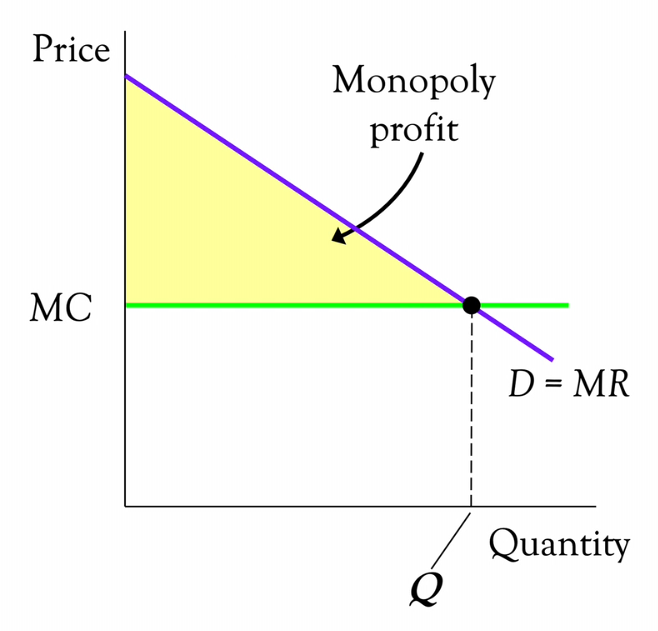
\includegraphics[width=16em]{images/price_discrimination.png}
			\centering
		\end{figure}
	    \item Harford The Undercover Economist Chapter 2: \textit{What Supermarkets Don't Want You to Know}
	    \begin{itemize}
	    	\item Unique target (first-degree)
	    	\item Group target (third-degree)
	    	\item Self-incrimination
	    \end{itemize}
	\end{itemize}
\end{itemize}
\subsection{Monopolistic Competition}
\begin{itemize}
	\item \textbf{Many} buyers and sellers
	\item Offer \textbf{differentiated} products
	\item Sellers are \textbf{free} to enter and exit the market
	\begin{itemize}
		\item LR Economic profit = 0 due to entry and exit
		\item New firms enter the market due to existing firms making profits
	\end{itemize}
    \item \impt \textbf{Externalities due to entry of new firms}
    \begin{itemize}
    	\item \textbf{Product-variety externality}: consumers benefit from intro of new products
    	\item \textbf{Business-stealing externality}: existing firms lose revenues when new firms enter the market
    \end{itemize}
\end{itemize}
\subsection{Oligopoly}
\begin{itemize}
	\item \textbf{N-firm Concentration Ratio}: percentage of the market's total output supplied by the N largest firms
	\item Only \textbf{a few} sellers offer similar or identical products
	\item A firm's decision about $P$ or $Q$ can affect other firms
	\begin{itemize}
		\item The firm will consider the reactions from other firms when making decisions
	\end{itemize}
    \item \textbf{Game theory}: study of how people behave in strategic situations
    \item \textbf{Types of oligopoly}
    \begin{itemize}
    	\item \underline{Collusion}: an agreement among firms in a market about quantities to produce or prices to charge
    	\item \underline{Cartel}: A group of firms acting in unison (e.g. price fixing)
    	\begin{itemize}
    		\item Cartel = Monopoly
    		\item Collective firms acting as a single unit, hence graph is equal to monopoly
    	\end{itemize}
    \end{itemize}
\end{itemize}
\subsubsection{Game Theory}
\textbf{Collusion vs self-interest}
\begin{itemize}
	\item Both firms would be better off if they both stick to the cartel agreement
	\item But each firm has an incentive to cheat
\end{itemize}
\textbf{Nash Equilibrium}
\begin{itemize}
	\item A situation in which players interacting with one another each chooses his best strategy given the strategies that all the others have chosen
\end{itemize}
\textbf{Dominant Strategy}
\begin{itemize}
	\item A strategy that is best for a player in a game regardless of the strategies chosen by the other players
\end{itemize}
\textbf{Prisoners' Dilemma}
\begin{itemize}
	\item Cooperation is difficult even when it is mutually beneficial
	\item Both players have dominant strategies that result in inefficient outcomes
	\begin{center}
		\begin{table}[H]
			\centering{
			\begin{tabular}{cc|cc}
				&  & \multicolumn{2}{c}{P2}     \\ \cline{3-4}
				&  & \multicolumn{1}{c|}{A} & B \\ \hline
				\multicolumn{1}{c|}{\multirow{2}{*}{P1}} &
				A &
				\multicolumn{1}{c|}{\begin{tabular}[c]{@{}c@{}}P1: Good\\ P2: Good\end{tabular}} &
				\begin{tabular}[c]{@{}c@{}}P1: Worst\\ P2: Best\end{tabular} \\ \cline{2-4}
				\multicolumn{1}{c|}{} &
				B &
				\multicolumn{1}{c|}{\begin{tabular}[c]{@{}c@{}}P1: Best\\ P2: Worst\end{tabular}} &
				\begin{tabular}[c]{@{}c@{}}P1: Bad\\ P2: Bad\end{tabular}
			\end{tabular}}
		\end{table}
	\end{center}
	\item Non-cooperative oligopoly equilibrium will be
	\begin{itemize}
		\item Bad for oligopoly firms: prevented from achieving \textbf{monopoly} profits
		\item Good for society: $Q$ is closer to the socially efficient output, $P$ is closer to MC
	\end{itemize}
    \item Strategies that lead to cooperation:
    \begin{itemize}
    	\item \textbf{Grim}:\\
    	Initially, a player using grim trigger will cooperate, but as soon as the opponent defects (thus satisfying the trigger condition), the player using grim trigger will defect for the remainder of the iterated game. Since a single defect by the opponent triggers defection forever, grim trigger is the most strictly unforgiving of strategies in an iterated game.
    	\item \textbf{Tit for Tat}\\
    	 For example, two competing economies can use a tit-for-tat strategy so that both participants benefit. One economy \textbf{starts with cooperation }by not imposing import tariffs on the other economy's goods and services to induce good behavior. The idea is that the second economy responds by also choosing not to impose import tariffs. If the second economy reacts by implementing tariffs, the first economy retaliates by implementing tariffs of its own to discourage the behavior.
    \end{itemize}
\end{itemize}
\end{multicols}









\end{document}